\maincolumn{
\vspace{-2.5cm}
\begin{center}
ARFC: \textbf{Advanced Reactors} and \textbf{Fuel Cycles}\\
\fontsizetitle
PI: {\textbf{Prof. Katy Huff}}, \href{mailto:kdhuff@illinois.edu}{\underline{kdhuff}@\underline{illinois.edu}}\\
\vspace{-2cm}\rule{\textwidth}{5pt}\vspace{2cm}
\end{center}

\fontsizesection
\begin{tikzpicture}
\iftrue
\node (multiphysics) [main, xshift=-3cm] {
\textcolor{black}{
\newline{\fontsizetitle Coupled Multiphysics of Advanced Reactors}\\
\vspace{-25pt}\rule{\textwidth}{5pt}\\
\fontsizesection
\vspace{.5cm}
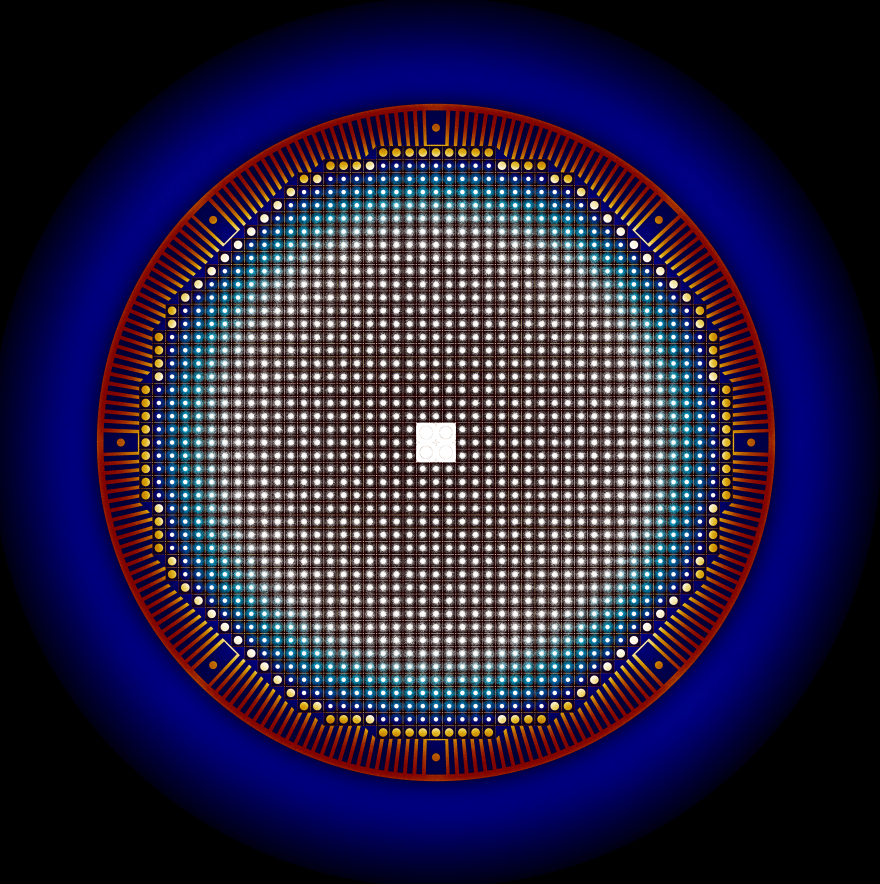
\includegraphics[width = \textwidth]{img/multiphysics.png}\\
}
};
\node (fuelcycle) [main, right of = multiphysics, xshift = 17.65cm] {
\textcolor{black}{
\newline{\fontsizetitle Nuclear Fuel Cycle Analysis}\\
\vspace{-20pt}\rule{\textwidth}{5pt}\\
\fontsizesection
\vspace{1.5cm}
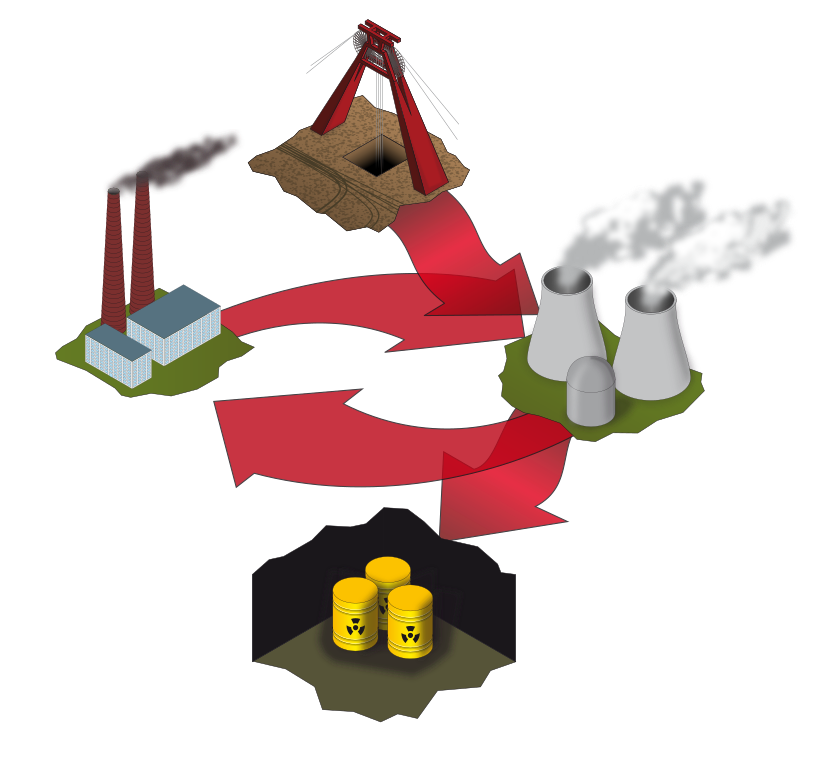
\includegraphics[width=\textwidth]{img/nfc.png}\\
\vspace{7pt}
}
};
\node (compute) [main, right of = fuelcycle, xshift = 17.65cm] {
\textcolor{black}{
\newline{\fontsizetitle Advanced Computation}\\
\vspace{-25pt}\rule{\textwidth}{5pt}\\
\fontsizesection
\vspace{17pt}
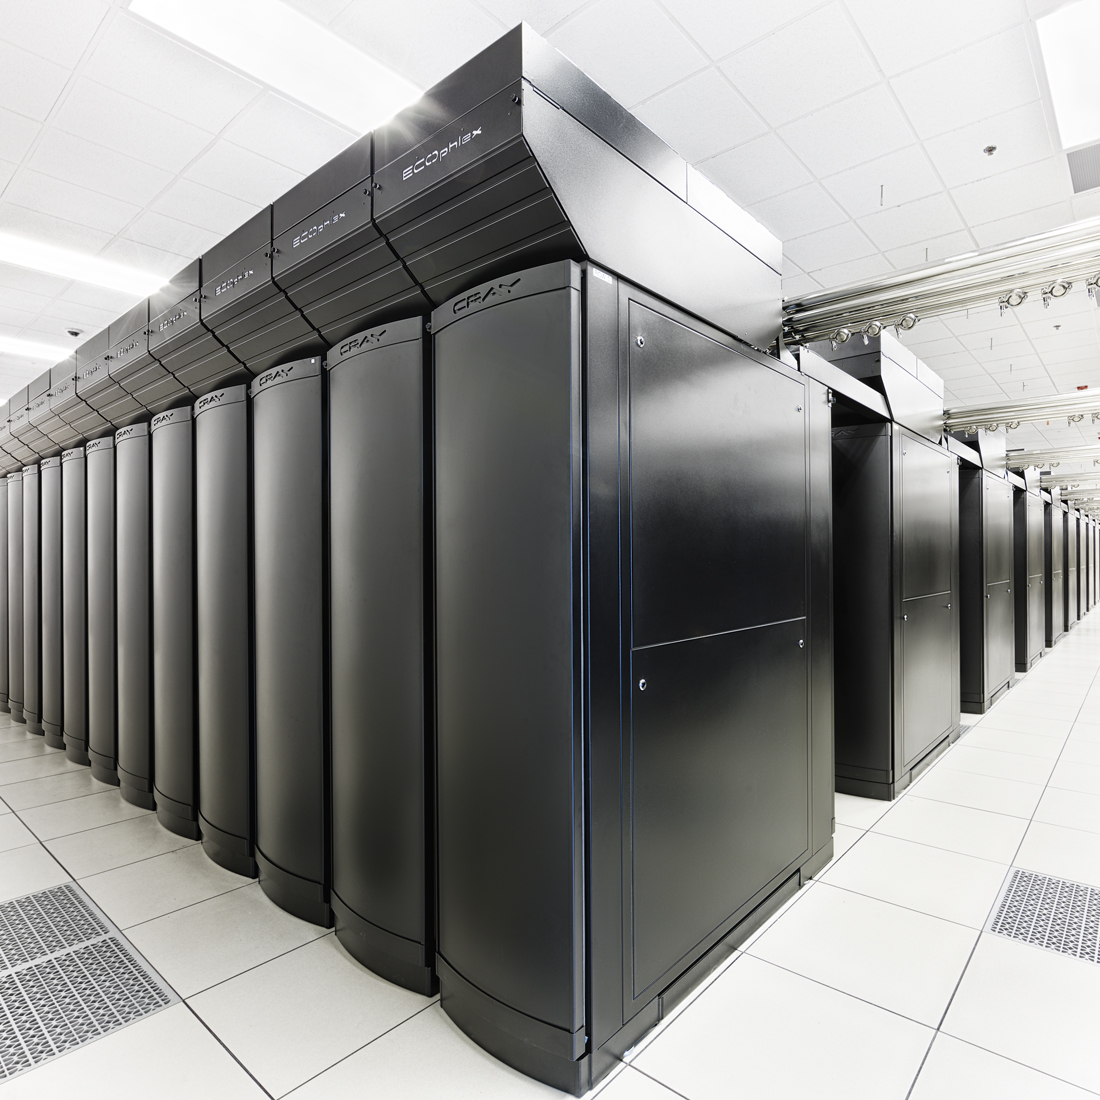
\includegraphics[width=\textwidth]{img/bw_cropped.jpg}\\
\vspace{5pt}
}
};
\fi
\iffalse
\node (diagram) [blurb, xshift = -3cm] {
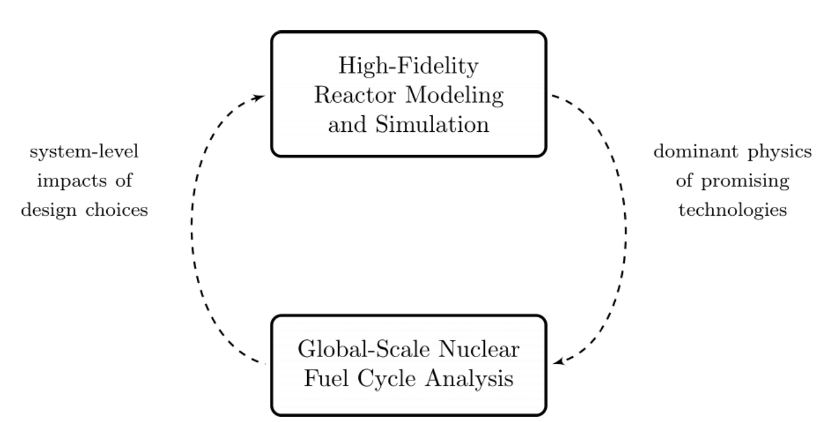
\includegraphics[width = \linewidth]{img/diagram.png}
};
%yshift is 21 for including this
\fi
\node (logos) [blurb, yshift = -19cm, xshift = -3cm] {\vspace{5pt}
\textcolor{black}{
\newline{\fontsizetitle Open-Source Nuclear Research Codes}\\
\vspace{-20pt}\rule{\textwidth}{5pt}\\
\vspace{25pt}
\begin{minipage}{.2\linewidth}
    
\includegraphics[width = \linewidth]{img/openmc_logo.png}\\
    \vspace{5pt}
    
\includegraphics[width = \linewidth]{img/rollo-logo.png}
\end{minipage} 
\begin{minipage}{.2\linewidth}
    
\includegraphics[width =.8\linewidth]{img/pyne.png}
    \vspace{10pt}
\end{minipage}
\begin{minipage}{.2\linewidth}
    
\includegraphics[width=.8\linewidth]{img/ghastly.png}
\end{minipage}
\begin{minipage}{.2\linewidth}
    
\includegraphics[width=\linewidth]{img/cyclus.png}\\
    \vspace{20pt}
    \textcolor{altgeldorange!100}{\textbf{\fontsizemoltres{\texttt{Moltres}}}}\\\vspace{-15pt}
\end{minipage}
}
};
\end{tikzpicture}

\vspace{1.5cm}
\begin{minipage}{.235\linewidth}
    \centering
    
\includegraphics[width=.8\linewidth]{img/qrcode.eps}
    \href{https://arfc.github.io/}{\fontsizesection\underline{https://arfc.github.io/}}
\end{minipage}
\vspace{-1cm}
\begin{minipage}{0.72\linewidth}
    \hspace{.5cm}
    \begin{tikzpicture}
    \vspace{-1cm}
        \node (logos) [blurb] {
        \begin{minipage}{.3\linewidth}
        `   %https://www.energy.gov/department-energy-logo-and-branding-guidelines
            
\includegraphics[width = \linewidth]{img/doe.png}
        \end{minipage}
        \begin{minipage}{.3\linewidth}
            %https://commons.wikimedia.org/wiki/File:NNSA_Logo.png
            
\includegraphics[width = \linewidth]{img/nnsa.png}
        \end{minipage}
        \begin{minipage}{.3\linewidth}
            % top left https://en.m.wikipedia.org/wiki/File:US-NuclearRegulatoryCommission-Logo.svg
            
\includegraphics[width = \linewidth]{img/nrc.png}
        \end{minipage}
        \vspace{1cm}
        \begin{minipage}{.3\linewidth}
        `   %https://www.moltexenergy.com/partners/ornl-logo/
            
\includegraphics[width = \linewidth]{img/ornl.png}
        \end{minipage}
        \begin{minipage}{.3\linewidth}
            %https://commons.wikimedia.org/wiki/File:Argonnelablogo.PNG
            
\includegraphics[width = \linewidth]{img/anl.png}
        \end{minipage}
        \begin{minipage}{.3\linewidth}
        \hspace{3.25cm}
            % https://inl.gov/logos-videos-images/
            
\includegraphics[height = .5\linewidth]{img/inl.png}
        \end{minipage}
        };
    \end{tikzpicture}
\end{minipage}

\vspace{2cm}
\begin{center}
    \begin{tcolorbox}[colback=white, colframe=black, width=0.9\textwidth, arc=6pt, boxrule=1pt]
        \bibliographystyle{plain}
        \bibliography{group-poster}
    \end{tcolorbox}
\end{center}
}{
}